% 2000 年全国旧课程卷文科第 22 题：梯形、分点与双曲线
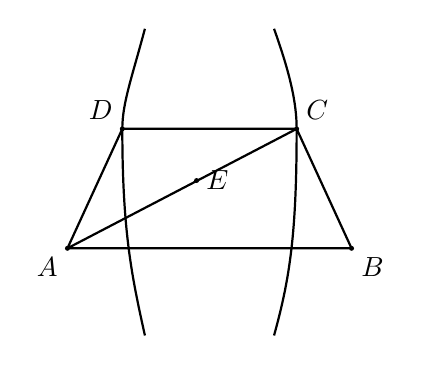
\begin{tikzpicture}[>=stealth, scale=0.82]
  \coordinate (A) at (0,0);
  \coordinate (B) at (4.4,0);
  \coordinate (D) at (0.85,1.85);
  \coordinate (C) at (3.55,1.85);
  \coordinate (E) at (2.0,1.05);

  \draw[thick] (A)--(B)--(C)--(D)--cycle;
  \draw[thick] (A)--(C);
  \draw[thick] (1.2,3.4) .. controls (1.0,2.65) and (0.85,2.25) .. (0.85,1.85);
  \draw[thick] (3.2,3.4) .. controls (3.45,2.7) and (3.55,2.25) .. (3.55,1.85);
  \draw[thick] (1.2,-1.35) .. controls (1.0,-0.45) and (0.85,0.25) .. (0.85,1.85);
  \draw[thick] (3.2,-1.35) .. controls (3.45,-0.45) and (3.55,0.25) .. (3.55,1.85);

  \fill (A) circle (1.1pt) node[below left] {$A$};
  \fill (B) circle (1.1pt) node[below right] {$B$};
  \fill (C) circle (1.1pt) node[above right] {$C$};
  \fill (D) circle (1.1pt) node[above left] {$D$};
  \fill (E) circle (1.1pt) node[right] {$E$};
\end{tikzpicture}
